% Created 2024-11-17 Sun 10:48
% Intended LaTeX compiler: pdflatex
\documentclass[12pt]{tiet-question-paper}
\usepackage{amsmath}
\usepackage{graphicx}
\usepackage{wrapfig}
\usepackage{amssymb}
\usepackage[unicode]{hyperref}


\usepackage{minted}
\hypersetup{%
colorlinks,%
breaklinks,%
urlcolor=[rgb]{0,0.35,0.65},%
linkcolor=[rgb]{0,0.35,0.65}%
}
\usepackage{libertinus}
\instlogo{images/tiet-logo.pdf}
\schoolordepartment{%
Computer Science \& Engineering Department}
\examname{Exercise (TTS) (2024-25 Odd)}
\coursecode{UCS749}
\coursename{Conversational AI: Speech Proc. […]}
\timeduration{2 hours}
\maxmarks{--}
\faculty{RGB}
\date{Nov 2024}
\title{}
\hypersetup{
 pdfauthor={B.V. Raghav},
 pdftitle={},
 pdfkeywords={},
 pdfsubject={},
 pdfcreator={Emacs 29.4 (Org mode 9.6.24)}, 
 pdflang={English}}
\begin{document}

\thispagestyle{empty}
\maketitle

\bvrskipline[-1.85]
\bvrhrule

\begin{enumerate}
\item If \(P_\theta\) models a data \(\mathcal{D}\) with an
intent of generating novel samples, \(\mathbf{x}\sim
   P_\theta\).  Is \(P_\theta\) a posterior distribution?
Comment. \hfill [2 marks]
\end{enumerate}

\bvrskipline[0.25]
\begin{enumerate}[resume]
\item If \(X\equiv\{\mathbf{x}_1,\ldots,\mathbf{x}_T\}\) is
a temporal sequence and each time step is
independently and identically distributed,
\begin{enumerate}
\item Prove that \(\log P(X) = \sum_{i=1}^T\log P(x_i)\);
\item If \(X\) is a Bernoulli process, \emph{i.e.} if each
\(x_{i}\) is a coin toss, with hit rate \(p\), the
log likelihood of \(k\) hits is \(k\log p +
      (T-k)\log (1-p)\).
\end{enumerate}
\end{enumerate}



\begin{center}
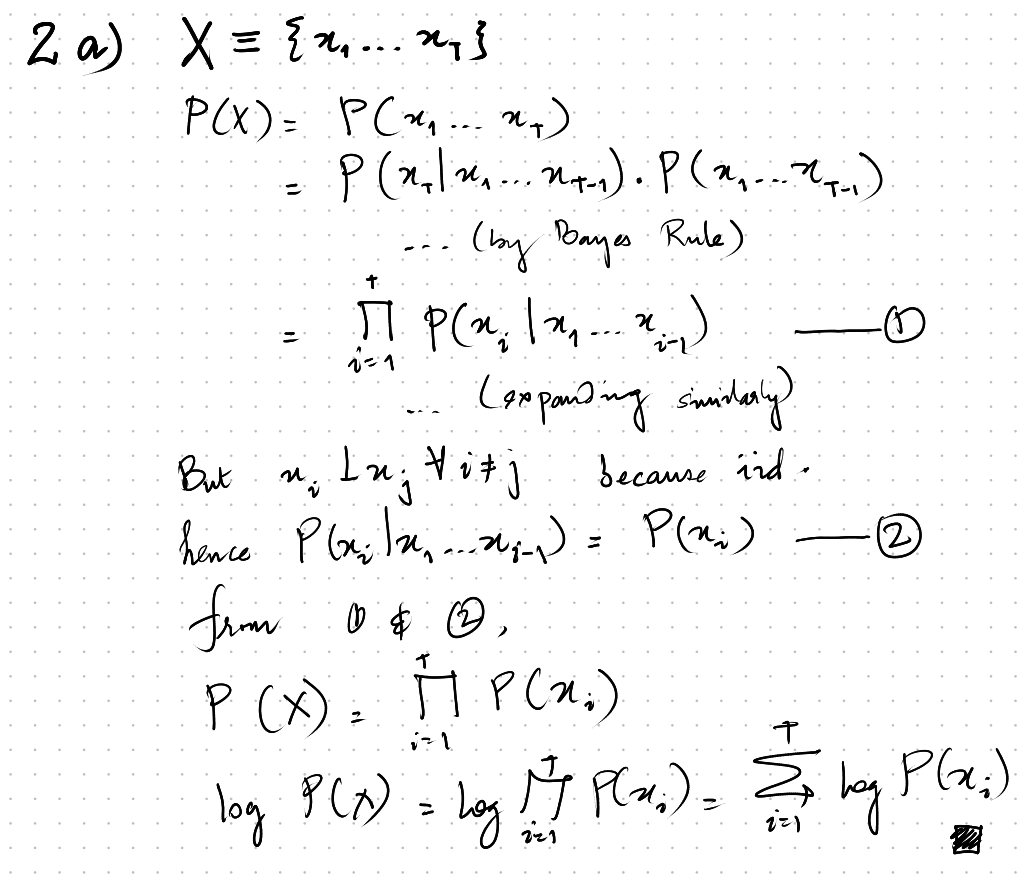
\includegraphics[width=.9\linewidth]{org-download-images/2024-11-12_10-15-18_screenshot.png}
\end{center}

\begin{center}
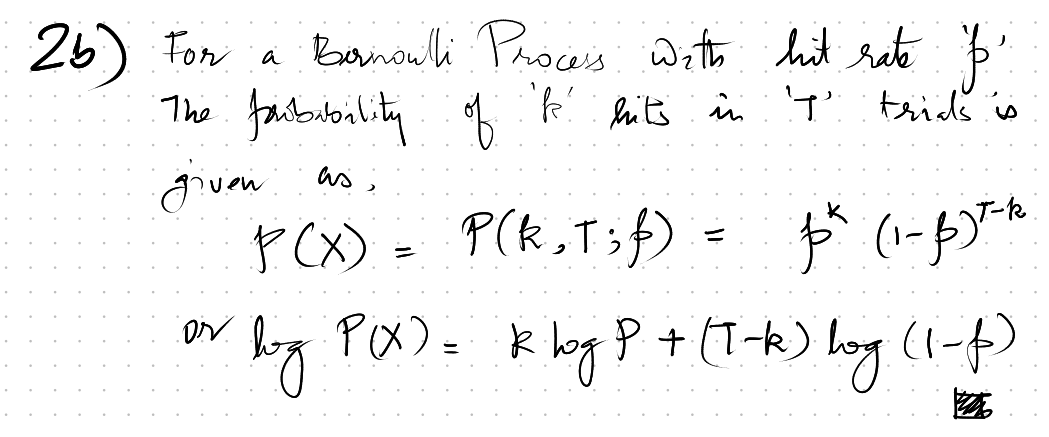
\includegraphics[width=.9\linewidth]{org-download-images/2024-11-12_10-18-39_screenshot.png}
\end{center}


\bvrskipline[0.25]
\begin{enumerate}[resume]
\item If \(X\equiv\{\mathbf{x}_1,\ldots,\mathbf{x}_T\}\) is
the temporal sequence of a Markov process, prove
that \(\log P(X) = \sum_{i=1}^T \log P(x_i\mid x_{i-1})\).
\end{enumerate}


\newpage
\bvrskipline[0.25]
{\huge

Speech sample \(X\) is a temporal sequence of intensities,

\begin{align*}
  X&\equiv\{x_1\ldots x_T\}
\end{align*}

Given speech samples \(\mathcal{D}\) as evidence,
estimate \(P_{\theta}\approx \mathcal{D}\) so that \(X\sim
P_\theta\) is a valid speech sample.

}

\newpage
\bvrhrule

{\huge

Let \(G_{\theta,\mathcal{N}} : \mathbb{X}^K \to
\mathbb{X}\) represent the model.

where,
\begin{itemize}
\item \(\mathbb{X}\) is the field of inputs.
\begin{itemize}
\item For a continuous model, \(\mathbb{X}\equiv
    \mathbb{R}\); whereas,
\item For categorical model,
\(\mathbb{X}\equiv\mathbb{R}_{[0,1]}^{256}\);
\item It may also be a hybrid model, \\[0pt]
\emph{e.g.} \(G_{\theta,\mathcal{N}} : \mathbb{R}^K \to
    \mathbb{R}_{[0,1]}^{256}\). \\[0pt]
Can you think how?
\end{itemize}
\end{itemize}

Let \(G_{\theta,\mathcal{N}} : \mathbb{X}^K \to
\mathbb{X}\) represent the model.

where,
\begin{itemize}
\item \(\mathcal{N}\) is a noise sampler,
\begin{itemize}
\item Generally, implemented as a normal distribution; or
\item Implemented implicitly as dropouts.
\end{itemize}
\end{itemize}

Let \(G_{\theta,\mathcal{N}} : \mathbb{X}^K \to
\mathbb{X}\) represent the model.

where,
\begin{itemize}
\item \(\theta\) are parameters of the model; and
\item \(\mathbf{x}_{t} = G_{\theta,\mathcal{N}}
  \left( \begin{bmatrix} \mathbf{x}_{t-K} & \ldots &
  \mathbf{x}_{t-1} \end{bmatrix} \right)\) models the
conditional distribution \(P(x_t \mid x_{t-K}\ldots
  x_{t-1})\)
\end{itemize}

\newpage

In case of Conditional Generation,

\(\mathbf{x}_{t} = G_{\theta,\mathcal{N}}
\left( \begin{bmatrix} \mathbf{x}_{t-K} & \ldots &
\mathbf{x}_{t-1} \end{bmatrix}, \mathbf{h} \right)\) \\[0pt]
models the conditional distribution \\[0pt]
\(P(x_t \mid x_{t-K}\ldots x_{t-1}, \mathbf{h})\)

\(\mathbf{h}\) represents the global conditions, \emph{e.g.}
\begin{itemize}
\item Text input;
\item Speaker;
\item Accent;
\item and so forth.
\end{itemize}

\newpage

Let \\[0pt]
\(X\equiv\begin{bmatrix} \mathbf{x}_1 & \ldots &
\mathbf{x}_T \end{bmatrix} \sim G_{\theta,\mathcal{N}}\)
be the output of the auto-regressive model, so that \\[0pt]
\(\mathbf{x}_{t} = G_{\theta,\mathcal{N}}
\left( \begin{bmatrix} \mathbf{x}_{t-K} & \ldots &
\mathbf{x}_{t-1} \end{bmatrix} \right)\)

\bvrskipline[0.25]

And, \\[0pt]
\(Y\equiv\begin{bmatrix} \mathbf{y}_1 & \ldots &
\mathbf{y}_T \end{bmatrix} \sim \mathcal{D}\) be a
speech sample from dataset.  Recall that for each time
step, the sound intensity is pre-processed so that the
values are remapped, quantised, and converted to
one-hot vectors, so that \(\mathbf{y}_t\in\{0,1\}^{256};
\|\mathbf{y}_t\|_{1}=1\) .

\bvrskipline[0.25]

The training objective is the cross entropy function,
given as,
\begin{align*}
  \underset{G}{\text{minimise}}\quad
  \underset{X\sim G, Y\sim\mathcal{D}}{\mathbb{E}}
  \left[ \sum_{i,t} y_{i,t}\log x_{i,t} \right]
\end{align*}


}

\vfill
\bvrhrule
\bvrskipline[-0.85]
\bvrhrule
\end{document}
